\section{TerraRanger Multiflex}
The TeraRanger Multiflex is a modular Time-of-Flight (ToF) (shown in Fig.~\ref{fig:terraMount}) sensor array designed for robotics applications, including SLAM and maze-solving. The system includes eight ToF sensors, a Multiflex Hub, flex cables, and connectors, enabling flexible deployment \cite{terra_mount}.

\begin{figure}[H]
	\centering
	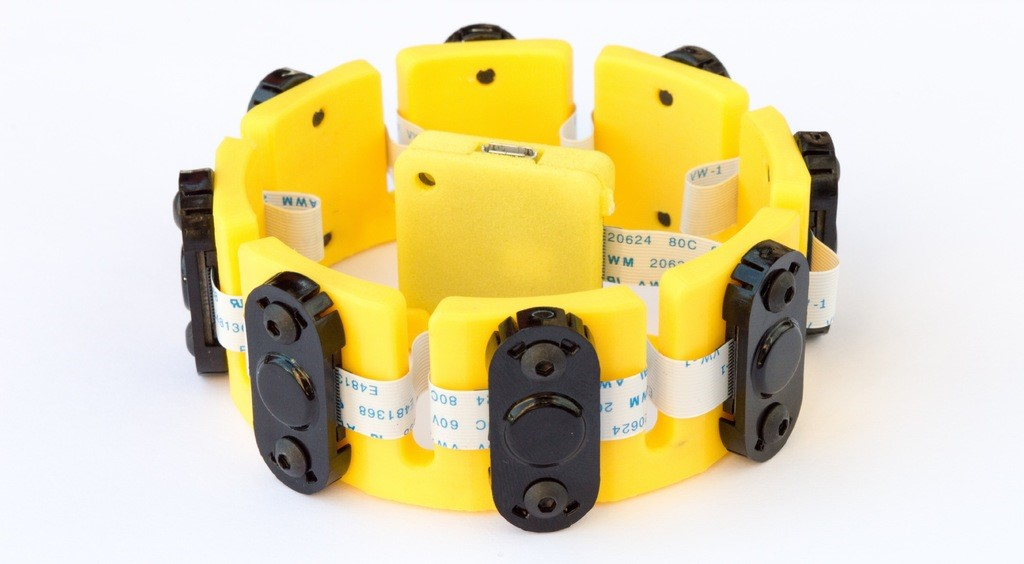
\includegraphics[height=6cm]{assets/terraRangerMultiplex.jpg}
	\caption{TeraRanger Multiflex circular mount \cite{terra_mount}.}
	\label{fig:terraMount}
\end{figure}

\textbf{Key Features and Considerations}
\begin{itemize}
	\item \textbf{Compact and Modular Design}: Each sensor is enclosed in a polycarbonate cover and can be mounted using M3 screws.
	\item \textbf{Safe Laser Emission}: The sensors utilize a low-power laser emitter; optical modifications are not recommended.
	\item \textbf{Stable Power Requirements}: Operates at 5V ±0.25V with minimal ripple and noise.
	\item \textbf{Reliable Connectivity}: Utilizes a 7-pin Hirose DF13 connector for UART/I2C communication; designed for robust vibration-resistant connections.
	\item \textbf{Mounting Precautions}: Avoid exposure to heat, dust, and strong electromagnetic fields for optimal performance.
\end{itemize}

\subsection{Connector and Data Interfaces}
\begin{figure}[H]
	\centering
	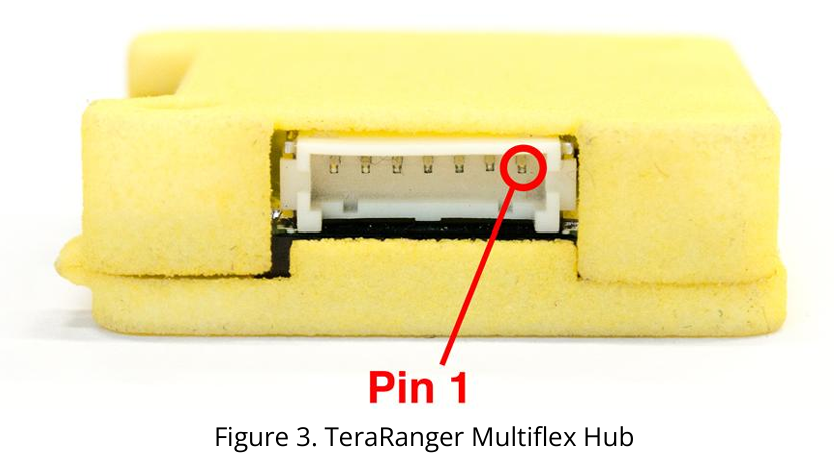
\includegraphics[height=3cm]{assets/TerraRangerMultflexHubPinout.png}
	\caption{TeraRanger Multiflex Hub pinout \cite{terra_mount}.}
	\label{fig:terraPinout}
\end{figure}

The \textbf{TeraRanger Multiflex Hub} connects to external equipment via a \textbf{7-pin Hirose DF13 connector} (female part: \textbf{DF13-7S-1.25C}). A compatible connector cable is included in the package. The pin configuration is as follows:

\begin{table}[H]
	\centering
	\begin{tabular}{|c|l|}
		\hline
		\textbf{Pin} & \textbf{Function} \\
		\hline
		7   & GND \\
		6   & RX Serial In (UART) \\
		5   & TX Serial Out (UART) \\
		4   & Interrupt Pin \\
		3   & SDA (I2C) \\
		2   & SCL (I2C) \\
		1   & 5 V Power Supply \\
		\hline
	\end{tabular}
	\caption{TeraRanger Multiflex Hub connector pinout}
	\label{tab:multiflex_pinout}
\end{table}

\subsection{UART Data Interface (Default)}
The \textbf{UART interface} operates at \textbf{3.3V output levels} (accepting inputs from \textbf{3.3V to 5V}). To connect the hub to a computer, a \textbf{USB-to-serial adapter} (e.g., FTDI breakout board) should be used. The default UART configuration is:

\begin{itemize}
	\item \textbf{Baud Rate:} 115200 bit/s
	\item \textbf{Data Bits:} 8
	\item \textbf{Parity:} None
	\item \textbf{Stop Bits:} 1
\end{itemize}

\subsection{I2C Data Interface}
The \textbf{I2C interface} allows the hub to function as a slave device, connecting to an I2C master. The default \textbf{I2C base address} is \textbf{0x55}, and only one \textbf{TeraRanger Multiflex} can be used per I2C bus. The signal levels are \textbf{3.3V}, and the \textbf{maximum bus speed is 400 kHz}. Integrated \textbf{1.5k Ohm pull-up resistors} ensure proper bus communication.

\subsection{USB Interface}
A \textbf{micro-USB} port provides both \textbf{power and data communication}. On \textbf{Linux and macOS}, the hub appears as a \textbf{virtual COM port} without additional drivers. On \textbf{Windows}, a driver must be installed from:  

\begin{center}
	\url{http://www.st.com/en/development-tools/stsw-stm32102.html}
\end{center}

After installation, reconnect the device to enable the COM port. The communication settings remain \textbf{115200-8N1}.

